\documentclass[hidelinks,12pt]{article}
\usepackage[left=0.25cm,top=1cm,right=0.25cm,bottom=1cm]{geometry}
%\usepackage[landscape]{geometry}
\textwidth = 20cm
\hoffset = -1cm
\usepackage[utf8]{inputenc}
\usepackage[spanish,es-tabla]{babel}
\usepackage[autostyle,spanish=mexican]{csquotes}
\usepackage[tbtags]{amsmath}
\usepackage{nccmath}
\usepackage{amsthm}
\usepackage{amssymb}
\usepackage{mathrsfs}
\usepackage{graphicx}
\usepackage{subfig}
\usepackage{standalone}
\usepackage[outdir=./Imagenes/]{epstopdf}
\usepackage{siunitx}
\usepackage{physics}
\usepackage{color}
\usepackage{float}
\usepackage{hyperref}
\usepackage{multicol}
%\usepackage{milista}
\usepackage{anyfontsize}
\usepackage{anysize}
%\usepackage{enumerate}
\usepackage[shortlabels]{enumitem}
\usepackage{capt-of}
\usepackage{bm}
\usepackage{relsize}
\usepackage{placeins}
\usepackage{empheq}
\usepackage{cancel}
\usepackage{wrapfig}
\usepackage[flushleft]{threeparttable}
\usepackage{makecell}
\usepackage{fancyhdr}
\usepackage{tikz}
\usepackage{bigints}
\usepackage{scalerel}
\usepackage{pgfplots}
\usepackage{pdflscape}
\pgfplotsset{compat=1.16}
\spanishdecimal{.}
\renewcommand{\baselinestretch}{1.5} 
\renewcommand\labelenumii{\theenumi.{\arabic{enumii}})}
\newcommand{\ptilde}[1]{\ensuremath{{#1}^{\prime}}}
\newcommand{\stilde}[1]{\ensuremath{{#1}^{\prime \prime}}}
\newcommand{\ttilde}[1]{\ensuremath{{#1}^{\prime \prime \prime}}}
\newcommand{\ntilde}[2]{\ensuremath{{#1}^{(#2)}}}

\newtheorem{defi}{{\it Definición}}[section]
\newtheorem{teo}{{\it Teorema}}[section]
\newtheorem{ejemplo}{{\it Ejemplo}}[section]
\newtheorem{propiedad}{{\it Propiedad}}[section]
\newtheorem{lema}{{\it Lema}}[section]
\newtheorem{cor}{Corolario}
\newtheorem{ejer}{Ejercicio}[section]

\newlist{milista}{enumerate}{2}
\setlist[milista,1]{label=\arabic*)}
\setlist[milista,2]{label=\arabic{milistai}.\arabic*)}
\newlength{\depthofsumsign}
\setlength{\depthofsumsign}{\depthof{$\sum$}}
\newcommand{\nsum}[1][1.4]{% only for \displaystyle
    \mathop{%
        \raisebox
            {-#1\depthofsumsign+1\depthofsumsign}
            {\scalebox
                {#1}
                {$\displaystyle\sum$}%
            }
    }
}
\def\scaleint#1{\vcenter{\hbox{\scaleto[3ex]{\displaystyle\int}{#1}}}}
\def\bs{\mkern-12mu}


\title{La función delta de Dirac \\ \large {Matemáticas Avanzadas de la Física}\vspace{-3ex}}

\author{M. en C. Gustavo Contreras Mayén}
\date{ }

\pagestyle{fancy}
\fancyhf{}
\rhead{Curso MAF}
\lhead{\leftmark}
\rfoot{\thepage}
\setlength{\headheight}{16pt}%


\begin{document}
\maketitle
\fontsize{14}{14}\selectfont
\tableofcontents
\newpage

%Referencia Kusse - Chapter 5

\section{Introducción.}

La función $\delta$ de Dirac es una función extraña pero útil que tiene muchas aplicaciones en ciencia, ingeniería y matemáticas. 
\par
La función $\delta$ fue propuesta en 1930 por Paul Dirac en el desarrollo del formalismo matemático de la mecánica cuántica. Necesitaba una función que fuera cero en todas partes, excepto en un solo punto, donde era discontinua y se comportaba como un pico infinitamente alto e infinitamente estrecho de área unitaria.
\par
Los matemáticos se apresuraron a señalar que, estrictamente hablando, no hay ninguna función que tenga estas propiedades. Pero Dirac supuso que sí, y procedió a utilizarlo con tanto éxito que se desarrolló una nueva rama de las matemáticas para justificar su uso. Esta área de las matemáticas se denomina \emph{teoría de funciones generalizadas} y desarrolla, con todo detalle, la base de la función $\delta$ de Dirac. Este tratamiento riguroso es necesario para justificar el uso de estas funciones discontinuas, pero para el físico las interpretaciones físicas más simples son igualmente importantes.

\section{Funciones singulares en física.}

Las situaciones físicas se modelan generalmente mediante ecuaciones y operaciones sobre funciones continuas. A veces, sin embargo, es útil considerar idealizaciones discontinuas, como la densidad de masa de una masa puntual o la fuerza de un impulso mecánico infinitamente rápido.
\par
Las funciones que describen estas ideas son obviamente extremadamente discontinuas, porque ellas y todas sus derivadas deben divergir. Por esta razón, a menudo se les llama \emph{funciones singulares}. La función $\delta$ de Dirac se desarrolló para describir funciones que involucran este tipo de discontinuidades y proporcionar un método para manejarlas en ecuaciones que normalmente solo involucran funciones continuas.

\subsection{El impulso ideal.}

A menudo, el primer encuentro de un estudiante de física con la función $\delta$ es el impulso \enquote{ideal}.
\par
En mecánica, un impulso es una fuerza que actúa sobre un objeto durante un período de tiempo finito. Considera la fuerza realista representada en la figura (\ref{fig:f1}).

\begin{figure}[H]
\centering
\subfloat[]{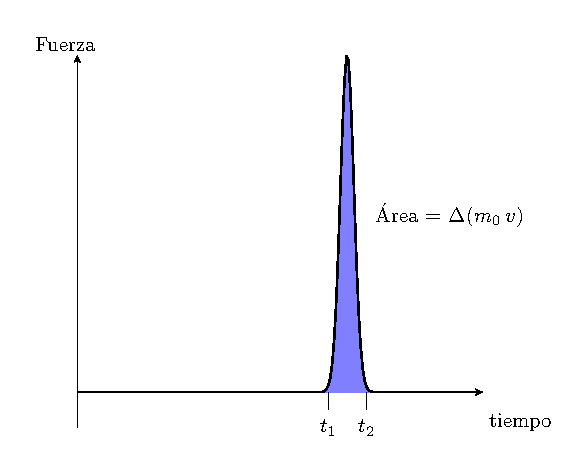
\includegraphics[width=0.5\textwidth]{Imagenes/delta_Dirac_Momento_00.eps}\label{fig:f1}}
\subfloat[]{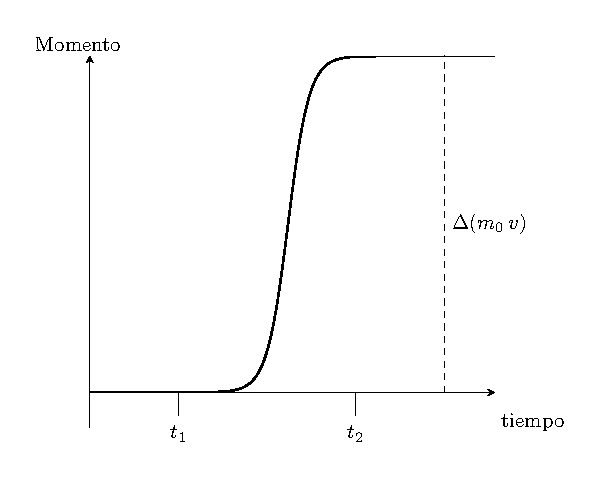
\includegraphics[width=0.5\textwidth]{Imagenes/delta_Dirac_Momento_01.eps}\label{fig:f2}}
\caption{Cambio en la fuerza y momento.}
\end{figure}

Vale cero hasta $t = t_{1}$, cuando aumenta suavemente desde cero hasta su valor máximo, y luego finalmente regresa a cero en $t = t_{2}$. Cuando esta fuerza se aplica a un objeto de masa $m_{0}$, el momento en la dirección de la fuerza aplicada cambia, como se muestra en la figura (\ref{fig:f2}).
\par
La cantidad de movimiento permanece constante hasta $t = t_{1}$, cuando comienza a cambiar continuamente hasta alcanzar su valor final en $t = t_{2}$. El cambio neto en el momento $\Delta (m_{0} \, v)$ es igual al área debajo de la curva de la fuerza:
\begin{align}
\begin{aligned}
\int_{-\infty}^{\infty} F(t) \dd{t} &= \int_{t_{1}}^{t_{2}} F(t) \dd{t} = \\[0.5em]
&= \int_{t_{1}}^{t_{2}} m_{0} \dv{v}{t} \dd{t} = \\[0.5em]
&= m_{0} \, v \, \eval_{t_{2}} - m_{0} \, v \, \eval_{t_{1}} = \\[0.5em]
&= \Delta (m_{0} \, v) 
\end{aligned}
\label{eq:ecuacion_05_01}
\end{align}

Un impulso ideal genera todo su cambio de momento instantáneamente, en el único punto $t = t_{0}$, como se muestra en la figura (\ref{fig:f2_1}). Por supuesto, que esto no es muy realista, ya que se requiere una fuerza infinita para cambiar el momento de una masa finita en un tiempo \enquote{cero}. Pero es un experimento mental aceptable, porque podríamos estar considerando el límite en el que un proceso físico ocurre más rápido de lo que cualquier medición puede detectar.

\begin{figure}[H]
    \centering
\subfloat[]{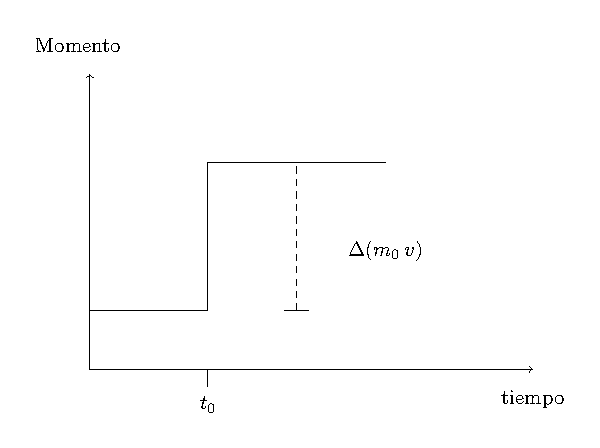
\includegraphics[width=0.5\textwidth]{Imagenes/delta_Dirac_Momento_02.eps}\label{fig:f2_1}}
\subfloat[]{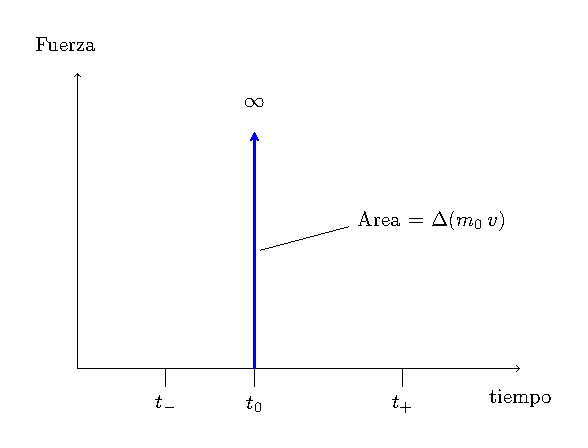
\includegraphics[width=0.5\textwidth]{Imagenes/delta_Dirac_Momento_03.eps}\label{fig:f2_2}}
\caption{Cambio instantáneo en el momento.}
\end{figure}    

La fuerza de un impulso ideal no puede graficarse como función del tiempo en el sentido normal. La fuerza existe solo por un instante, y por lo tanto vale cero en todas partes, excepto en $t = t_{0}$, cuando es infinita. Pero esto no es un infinito cualquiera. Dado que el cambio total de momento debe ser $\Delta (m_{0} \, v)$, la fuerza debe divergir para que su área bajo la curva cumpla (para todo $(t_{-} < t_{+})$:
\begin{align}
\int_{t_{-}}^{t_{+}} F(t) \dd{t} = \begin{cases}
\Delta (m_{0} \, v) & t_{-} < t_{+} \\
0 & \mbox{en otro valor}
\end{cases}
\label{eq:ecuacion_05_02}
\end{align}

En otras palabras, cualquier integral que incluya el punto $t_{0}$ da un cambio de momento de $\Delta (m_{0} \, v)$. Por otro lado, las integrales que excluyen a $t_{0}$ no deben dar ningún cambio de momento. Graficamos esto simbólicamente como se muestra en la figura (\ref{fig:f2_2}). Un pico de ancho cero con una flecha indica que la función va al infinito, mientras que el área del impulso generalmente se indica mediante un comentario en el gráfico, como se muestra en la figura, o algunas veces por la altura de la flecha.
\par
La función $\delta$ de Dirac $\delta (t)$ fue diseñada para representar exactamente este tipo de función \enquote{patológica}. La $\delta (t)$ vale cero en todas partes, excepto en $t = 0$, cuando es infinito. De nuevo, esto no es cualquier infinito. Diverge de tal manera que cualquier integral que incluya $t = 0$ tiene el valor de $1$, es decir (para todo $t_{-} < t_{+}$):
\begin{align}
\int_{t_{-}}^{t_{+}} \delta (t) \dd{t} = \begin{cases}
1 & t_{-} < t_{+} \\
0 & \mbox{en otro valor}
\end{cases}
\label{eq:ecuacion_05_03}
\end{align}
\noindent
De manera simbólica la gráfica de la función $\delta (t)$ se muestra en la figura (\ref{fig:figura_05_03}). 
\begin{figure}[H]
    \centering
    \includegraphics[scale=1.3]{Imagenes/delta_Dirac_Momento_05.eps}
    \caption{La función delta de Dirac $\delta (t)$}
    \label{fig:figura_05_03}
\end{figure}

El impulso ideal, discutido previamente, puede expresarse en términos de la función delta de Dirac desplazada:
\begin{align}
F(t) = \Delta (m_{0} \, v) \, \delta (t - t_{0})
\label{eq:ecuacion_05_04}
\end{align}
El argumento $t - t_{0}$ simplemente traduce el pico de la función para que ocurra en $t_{0}$ en lugar de $0$.

\subsection{Masas y cargas puntuales.}

En la física a menudo las ecuaciones involucran la masa por unidad de volumen $\rho_{m} (\va{r})$ en una región del espacio. Normalmente, $\rho_{m} (\va{r})$ es una función continua de posición, pero con la función $\delta$, también puede representar masas puntuales.
\par
Una masa puntual tiene una cantidad finita de masa dentro de un solo punto del espacio, por lo que la densidad debe ser infinita en ese punto y cero en cualquier otro lugar.
\par
Integrando la densidad de masa en un volumen $V$, se obtiene la masa total contenida:
\begin{align}
\int_{V} \rho_{m} (\va{r}) \dd{\tau} = \mbox{ masa total dentro de } V
\label{eq:ecuacion_05_05}
\end{align}
Así, si hay un solo punto de masa $m_{0}$, ubicado en el origen, como se muestra en la figura (\ref{fig:figura_05_04}), cualquier integral de volumen que incluya el origen debe dar la masa total como $m_{0}$, las integrales que excluyen el origen deben devolver cero. 
\begin{figure}[H]
    \centering
    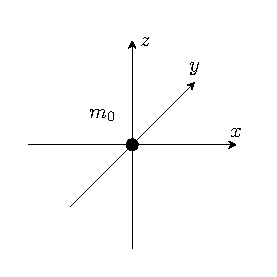
\includegraphics[scale=1.3]{Imagenes/delta_Dirac_Masa_Puntual.eps}
    \caption{Una masa puntual en el origen.}
    \label{fig:figura_05_04}
\end{figure}

En términos matemáticos:
\begin{align}
\int_{V} \rho_{m} (\va{r}) \dd{\tau} = \begin{cases}
m_{0} & \mbox{origen incluido en } V \\
0 & \mbox{origen excluido en } V
\end{cases}
\label{eq:ecuacion_05_06}
\end{align}

Usando la función $\delta$ de Dirac, la función densidad de masa es:
\begin{align}
\rho_{m} (\va{r}) = m_{0} \, \delta(x) \, \delta(y) \, \delta(z)
\label{eq:ecuacion_05_07}
\end{align}

La ec. (\ref{eq:ecuacion_05_06}) se puede verificar fácilmente expandiendo la integral como:
\begin{align}
\int_{V} \rho_{m} (\va{r}) \dd{\tau} = \iiint m_{0} \, \delta(x) \, \delta(y) \, \delta(z) \dd{x} \dd{y} \dd{z}
\label{eq:ecuacion_05_08}
\end{align}

Aplicar la ec. (\ref{eq:ecuacion_05_03}) a las tres integrales independientes devuelve $m_{0}$, solo cuando $V$ incluye el origen. Si, en lugar del origen, la masa puntual está ubicada en el punto $(x_{0}, y_{0}, z_{0})$, se utilizan argumentos desplazados en cada una de las funciones $\delta$:
\begin{align}
\rho_{m} (\va{r}) = m_{0} \, \delta (x - x_{0}) \, \delta (y - y_{0}) \, \delta (z - z_{0})
\label{eq:ecuacion_05_09}
\end{align}

\section{Dos definiciones de \texorpdfstring{$\delta (t)$}{d(t)}}

Hay dos formas comunes de definir la función $\delta$ de Dirac. El enfoque más riguroso, desde la teoría de funciones generalizadas, lo define por su comportamiento dentro de las operaciones integrales. De hecho, nunca se supone que la función $\delta$ exista fuera de una integral. En general, en ciencia e ingeniería se un poco más laxos y usan una segunda definición. A menudo definen la función $\delta$ como el límite de una secuencia infinita de funciones continuas. Además, como se demostró en los dos ejemplos anteriores, con frecuencia manipulan la función $\delta$ fuera de las integrales. Por lo general, no hay problemas con este enfoque menos riguroso.

\subsection{La función \texorpdfstring{$\delta(t)$}{d(t)} como límite de una secuencia.}

La función $\delta$ puede verse como el límite de una secuencia de funciones, es decir:
\begin{align}
\delta(t) = \lim_{n \to \infty} \delta_{n} (t)
\label{eq:ecuacion_05_10}
\end{align}
donde $\delta_{n}(t)$ es finito para todos los valores de $t$.
\par
Hay muchas secuencias de funciones que se acercan a la función $\delta$ de Dirac de esta manera. La más simple es la secuencia de función cuadrada definida por:
\begin{align}
\delta_{n} (t) = \begin{cases}
n & -\dfrac{1}{2 \, n} < t < \dfrac{1}{2 \, n} \\
0 & \mbox{en cualquier otro punto}
\end{cases}
\label{eq:ecuacion_05_11}
\end{align}
como se muestra en la figura (\ref{fig:figura_05_06}).
\begin{figure}[H]
    \centering
    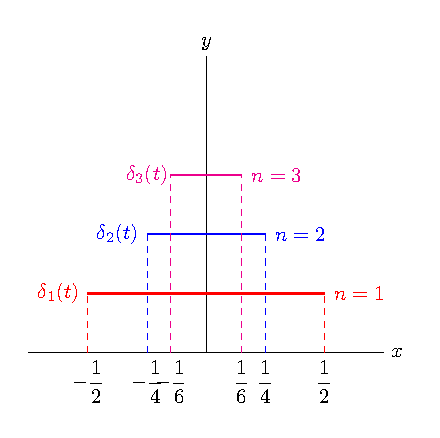
\includegraphics[scale=1.3]{Imagenes/plot_secuencia_delta_02.eps}
    \caption{Primeras tres funciones de la secuencia.}
    \label{fig:figura_05_06}
\end{figure}
Es claro que para cualquier valor de $n$:
\begin{align}
\int_{-\infty}^{\infty} \delta_{n} (t) \dd{t} = 1
\label{eq:ecuacion_05_12}
\end{align}
en el límite cuando $n \to \infty$, $\delta_{n}(t) = 0$ para todo valor de $t$, excepto $t = 0$. 
\par
Hay otras tres secuencias de funciones comunes que se acercan a la función $\delta$ de Dirac: las secuencias de resonancia, gaussiana y sinc al cuadrado, se muestran en las figuras (\ref{fig:figura_05_07}) a (\ref{fig:figura_05_09}) y se describen matemáticamente mediante:
\begin{align}
\begin{aligned}
\mbox{Resonancia:} \hspace{1cm} \delta_{n}(t) &= \dfrac{n/\pi}{1 + n^{2} \, t^{2}} \\[0.5em]
\mbox{Gaussiana:} \hspace{1cm} \delta_{n}(t) &= \dfrac{n}{\sqrt{\pi}} \, e^{-n^{2} t^{2}} \\[0.5em]
\mbox{Sinc cuadrada:} \hspace{1cm} \delta_{n}(t) &= \dfrac{\sin^{2} n \, t}{n \, \pi \, t^{2}} 
\end{aligned}
\label{eq:ecuacion_05_13}
\end{align}

\begin{figure}[H]
    \centering
    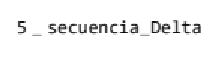
\includegraphics[scale=1.4]{Imagenes/secuencia_Delta_05.eps}
    \caption{Gráfica de la secuencia delta para la función resonancia.}
    \label{fig:figura_05_07}
\end{figure}

Cada una de esas funciones tiene un área unitaria para cualquier valor de $n$, y es fácil calcularla cuando en el límite $n \to \infty$, $\delta_{n} (t) = 0$ para todo $t \neq 0$.

\begin{figure}[H]
    \centering
    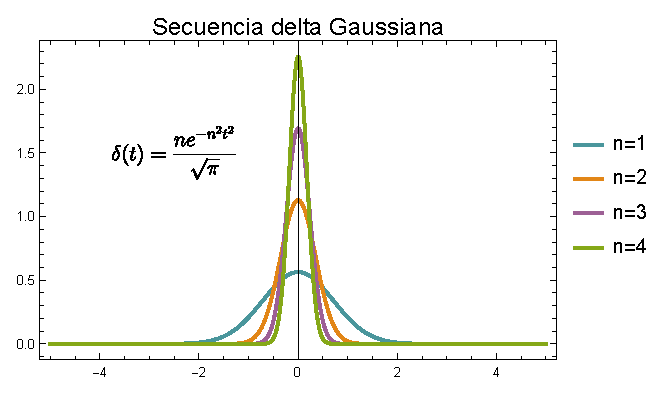
\includegraphics[scale=1]{Imagenes/secuencia_Delta_06.eps}
    \caption{Gráfica de la secuencia delta para la función Gaussiana.}
    \label{fig:figura_05_08}
\end{figure}

\begin{figure}[H]
    \centering
    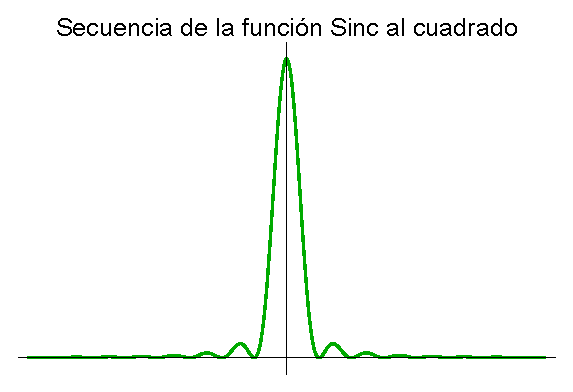
\includegraphics[scale=1]{Imagenes/secuencia_Delta_07.eps}
    \caption{Gráfica de la secuencia delta para la función sinc al cuadrado.}
    \label{fig:figura_05_09}
\end{figure}

\subsection{Definición de \texorpdfstring{$\delta(t)$}{d(t)} por operaciones integrales.}

En matemáticas, la función $\delta$ se define por cómo se comporta dentro de una integral. Cualquier función que se comporte como $\delta (t)$ en la siguiente ecuación es por definición una función $\delta$:
\begin{align}
\int_{t_{-}}^{t_{+}} f(t) \, \delta(t - t_{0}) \dd{t} = \begin{cases}
f(t_{0}) & t_{-} < t_{0}  < t_{+} \\
0 & \mbox{en cualquier otro punto}
\end{cases}
\label{eq:ecuacion_05_14}
\end{align}
donde $t_{-} < t_{+}$ y $f (t)$ es cualquier función continua de buen comportamiento. Esta operación a veces se denomina integral de filtrado, porque selecciona el valor único $f(t_{0})$ de $f(t)$.
\par
Debido a que esta es una definición, no es necesario probarla, pero se debe demostrar su coherencia con nuestra definición anterior y las aplicaciones de la función. Si $t_{-} < t_{0}  < t_{+}$, el rango de la integral se puede cambiar para que sea una región infinitesimal de tamaño $2 \, \varepsilon$ centrada alrededor de $t_{0}$, sin cambiar el valor de la integral. Esto es cierto porque $\delta (t - t_{0})$ se anula en todas partes excepto en $t = t_{0}$. Esto es:
\begin{align}
\int_{t_{-}}^{t_{+}} f(t) \, \delta (t - t_{0}) \dd{t} = \int_{t_{-} - \varepsilon}^{t_{+} + \varepsilon} f(t) \, \delta (t - t_{0}) \dd{t} 
\label{eq:ecuacion_05_15}
\end{align}
Como $f (t)$ es una función continua, sobre la región infinitesimal es efectivamente una constante, con valor $f(t_{0})$. Por lo tanto:
\begin{align}
\int_{t_{-}}^{t_{+}} f(t) \, \delta (t - t_{0}) \dd{t} = f(t_{0}) \, \int_{t_{-} - \varepsilon}^{t_{+} + \varepsilon} \delta (t - t_{0}) \dd{t} = f(t_{0})
\label{eq:ecuacion_05_16}
\end{align}
Esto \enquote{demuestra} la primera parte de la ec.(\ref{eq:ecuacion_05_14}) La segunda parte, cuando $t_{0}$  no está dentro del rango $t_{-} < t_{0}  < t_{+}$, se sigue fácilmente porque, en este caso, $\delta (t - t_{0})$ es cero para todo el rango del integrando.
\par
La figura () muestra una representación de la integración en la ec. (\ref{eq:ecuacion_05_14}). El integrando es un producto de una función de $\delta$ desplazada y la función continua $f (t)$. Debido a que la función $\delta$ es cero en todas partes excepto en $t = t_{0}$, el integrando va a una función $\delta$ ubicada en $t = t_{0}$, con un área escalada por el valor de $f (t_{0})$.
\begin{figure}[H]
    \centering
    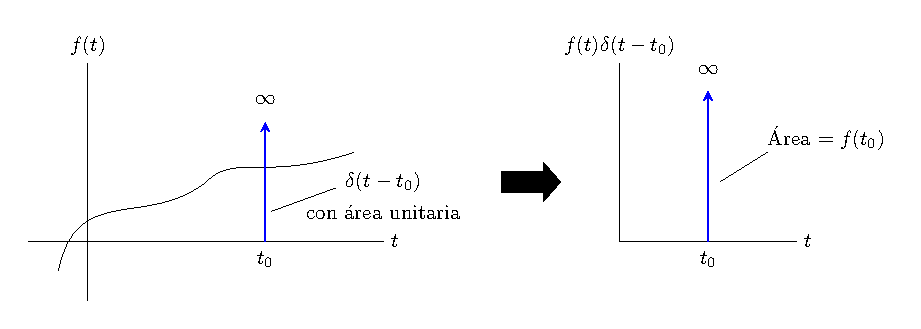
\includegraphics[scale=1]{Imagenes/plot_propiedad_desplazamiento.eps}
    \caption{Interpretación gráfica de la integral de filtro.}
    \label{fig:figura_05_10}
\end{figure}



\end{document}